% This is "sig-alternate.tex" V1.9 April 2009
% This file should be compiled with V2.4 of "sig-alternate.cls" April 2009
%
% This example file demonstrates the use of the 'sig-alternate.cls'
% V2.4 LaTeX2e document class file. It is for those submitting
% articles to ACM Conference Proceedings WHO DO NOT WISH TO
% STRICTLY ADHERE TO THE SIGS (PUBS-BOARD-ENDORSED) STYLE.
% The 'sig-alternate.cls' file will produce a similar-looking,
% albeit, 'tighter' paper resulting in, invariably, fewer pages.
%
% ----------------------------------------------------------------------------------------------------------------
% This .tex file (and associated .cls V2.4) produces:
%       1) The Permission Statement
%       2) The Conference (location) Info information
%       3) The Copyright Line with ACM data
%       4) NO page numbers
%
% as against the acm_proc_article-sp.cls file which
% DOES NOT produce 1) thru' 3) above.
%
% Using 'sig-alternate.cls' you have control, however, from within
% the source .tex file, over both the CopyrightYear
% (defaulted to 200X) and the ACM Copyright Data
% (defaulted to X-XXXXX-XX-X/XX/XX).
% e.g.
% \CopyrightYear{2007} will cause 2007 to appear in the copyright line.
% \crdata{0-12345-67-8/90/12} will cause 0-12345-67-8/90/12 to appear in the copyright line.
%
% ---------------------------------------------------------------------------------------------------------------
% This .tex source is an example which *does* use
% the .bib file (from which the .bbl file % is produced).
% REMEMBER HOWEVER: After having produced the .bbl file,
% and prior to final submission, you *NEED* to 'insert'
% your .bbl file into your source .tex file so as to provide
% ONE 'self-contained' source file.
%
% ================= IF YOU HAVE QUESTIONS =======================https://github.com/Boidkan/Senior_seminar_templates.git
% Questions regarding the SIGS styles, SIGS policies and
% procedures, Conferences etc. should be sent to
% Adrienne Griscti (griscti@acm.org)
%
% Technical questions _only_ to
% Gerald Murray (murray@hq.acm.org)
% ===============================================================
%
% For tracking purposes - this is V1.9 - April 2009

\documentclass{sig-alternate}
\usepackage{color}


%%%% User-defined macros
\newcommand{\lam}{\lambda}
\newcommand{\mycomment}[1]{\textcolor{red}{#1}}
%%%%% Uncomment this line (and comment the previous one)
%%%%% to remove all comments
%%%%% NOTE: comments still occupy a line even if invisible;
%%%%% Don't write them as a separate paragraph
%\newcommand{\mycomment}[3]{}
%\linespread{2}
\begin{document}

%
% --- Author Metadata here ---
\conferenceinfo{UMM CSci Senior Seminar Conference, April 2014}{Morris, MN}
%\CopyrightYear{2007} % Allows default copyright year (200X) to be over-ridden - IF NEED BE.
%\crdata{0-12345-67-8/90/01}  % Allows default copyright data (0-89791-88-6/97/05) to be over-ridden - IF NEED BE.==
% --- End of Author Metadata ---

\title{Applying Genetic Programming to \\ Bytecode and Assembly}
%\subtitle{[Extended Abstract]
%
% You need the command \numberofauthors to handle the 'placement
% and alignment' of the authors beneath the title.
%
% For aesthetic reasons, we recommend 'three authors at a time'
% i.e. three 'name/affiliation blocks' be placed beneath the title.
%
% NOTE: You are NOT restricted in how many 'rows' of
% "name/affiliations" may appear. We just ask that you restrict
% the number of 'columns' to three.
%
% Because of the available 'opening page real-estate'
% we ask you to refrain from ElenaSampleputting more than six authors
% (two rows with three columns) beneath the article title.
% More than six makes the first-page appear very cluttered indeed.
%
% Use the \alignauthor commands to handle the names
% and affiliations for an 'aesthetic maximum' of six authors.
% Add names, affiliations, addresses for
% the seventh etc. author(s) as the argument for the
% \additionalauthors command.
% These 'additional authors' will be output/set for you
% without further effort on your part as the last section in
% the body of your article BEFORE References or any Appendices.
\numberofauthors{1} %  in this sample file, there are a *total*
% of EIGHT authors. SIX appear on the 'first-page' (for formatting
% reasons) and the remaining two appear in the \additionalauthors section.
%
\author{
% You can go ahead and credit any number of authors here,
% e.g. one 'row of three' or two rows (consisting o
% and a second row of one, two or three).
%
% The command \alignauthor (no curly braces needed) should
% precede each author name, affiliation/snail-mail address and
% e-mail address. Additionally, tag each line of
% affiliation/address with \affaddr, and tag the
% e-mail address with \email.
%
% 1st. author
\alignauthor
Eric C. Collom \\
\affaddr{University of Minnesota, Morris} \\
\email{coll0474@morris.umn.edu}
}

\maketitle
\begin{abstract}
Traditional genetic programming (GP) has not yet been able to perform unrestricted evolution on entire programs at the source code level. Instead only small sections within the programs are usually evolved. Not being able to evolve whole programs is an issue since it limits the flexibility on what can be evolved. Evolving programs in either bytecode or assembly language is a method that has been used to perform unrestricted evolution. This paper provides an overview of applying genetic programming to Java bytecode and x86 assembly. Two examples of how this method can be implemented will be explored. We will also discuss experimental results that include evolving recursive functions and automated bug repair.
\end{abstract}


\keywords{evolutionary computation, x86 assembly code, Java bytecode, FINCH, automated bug repair}

\section{Introduction}
GP is a set of techniques used to automate computer problem solving. This is done by evolving programs with an evolutionary algorithm (EA) that imitates natural selection in order to find a solution. Traditional GP has commonly been used to evolve specific parts of programs instead of full-fledged programs. This is because traditionally we have to understand the structure of the program being evolved. An EA is usually designed for a specific program with knowledge about how the program works. Being able to evolve an entire program without knowing its structure would allow for more flexibility in GP. Evolving bytecode and assembly, instead of source code, is a method that allows for this flexibility. This is possible because bytecode and assembly languages are less restrictive syntactically than source code. We discuss this issue further in Section 3.\par 

Orlov and Sipper~\cite{FINCH2:2009} propose a method for applying GP to full-fledged programs that requires a program to be in Java bytecode. Schulte et al.,~\cite{Assembly:2010} apply a similar method with both Java bytecode and x86 assembly. Orlov and Sipper~\cite{FINCH:2011} focused on evolving simple programs as a whole while Schulte et al.,~\cite{Assembly:2010} focused on automated bug repair in programs.\par
	
This paper is organized as follows: Section 2 covers the background needed for understanding the application of GP to bytecode and assembly. It contains information on Evolutionary Computation (EC), Java bytecode, and the Java Virtual Machine. Section 3 describes the benefits of evolving assembly and bytecode. Section 4 discusses how Orlov and Sipper~\cite{FINCH:2011} evolved Java bytecode. Section 5 explores how Schulte, et al.,~\cite{Assembly:2010} evolved both x86 assembly and Java bytecode. Section 6 summarizes some of the experimental results from \cite{FINCH:2011} and \cite{Assembly:2010}.  Possible future work and ideas is also discussed.  
	
	

\section{Background}


This section explores the components of EC and GP. Java bytecode will also be discussed in addition to various details of the Java Virtual Machine (JVM). This section will only address Java bytecode since knowledge of x86 assembly is not needed to understand the research done by Schulte et al.,~\cite{Assembly:2010}. Also, throughout the rest of this paper, the term \textit{instruction-level code} will be used when referring to either Java bytecode or x86 assembly.
\subsection{Evolutionary Computation}
\begin{figure}
\centering
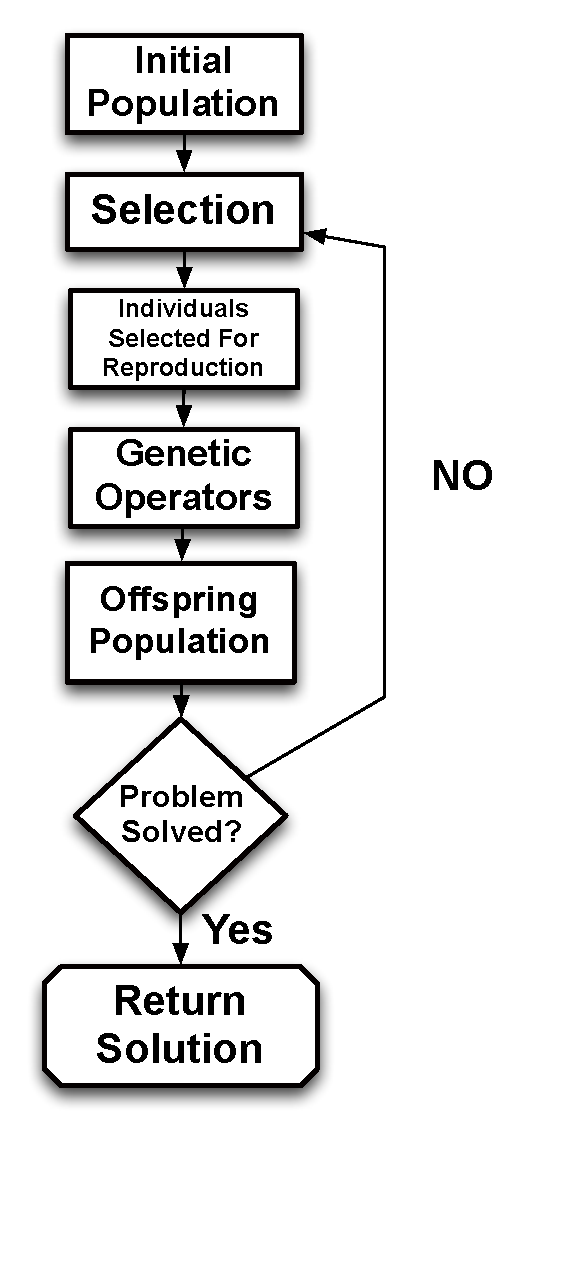
\psfig{file=ECdiagram.pdf,height=3in}

\caption{The process of Evolutionary Computation}
\label{ECdiagram}
\end{figure}


EC is a field of computer science and artificial intelligence that is loosely based on evolutionary biology. EC imitates evolution through continuous optimization in order to solve problems. Optimization in EC, in the best case scenario, is the selection of a few the best individuals within a population. The representation of what an individual is depends on the problem being solved. For example, it can be a string of bits, a parse tree, or an object. In this paper, the individuals will be programs in Java bytecode and x86 assembly.\par 

The EC process is summarized in Figure~\ref{ECdiagram}. An initial population of individuals is generated and a selection process is used to choose the most fit individuals. The selection process gives a fitness value, usually numerical, to each individual which indicates how well it solves the specific problem. For the research discussed in this paper a higher fitness indicates a more fit individual. The individuals with the highest fitness are then taken and modified using genetic operators that imitate mutation and sexual reproduction. A check is then done to see if any individuals from the new population solve the desired problem or a predetermined number of generations is reached. If not, the process of evolution is repeated.  If the problem is solved the individual with the best solution is returned.\par

	GP is a tool that uses the EC process to evolve programs. In the research discussed in this paper, the selection of individuals for sexual reproduction is done through tournament selection. A certain number of individuals are chosen for a simulated competition and the individual with the highest fitness wins. That individual is then selected to be a parent.\par 
		
	One way sexual reproduction is simulated in GP is through the genetic operator called crossover. Crossover is the process of taking two parent individuals and extracting a section of code from one and then replacing it with a section from the other program, to form an offspring. Mutation is another genetic operator that is used to produce offspring. Mutation takes a program and performs random changes on a randomly chosen section.


\subsection{Java Bytecode and the JVM}

\begin{figure}
\centering
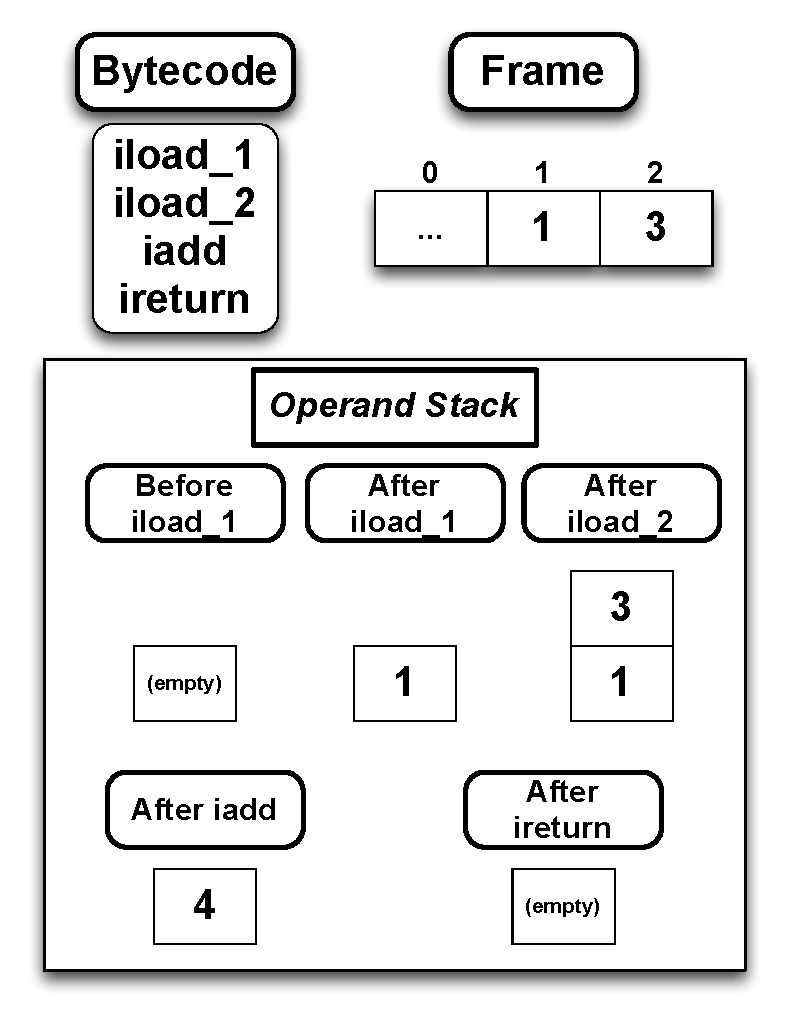
\psfig{file=stackBytecode.pdf,height=2.5in}

\caption{In this example we are assuming that the frame already contains the local variables 1 and 3 to retain simplicity. When \texttt{iload\_1} is executed, it takes the element from the frame at index 1 and pushes it onto the stack. \texttt{iload\_2} does the same thing but with index 2. \texttt{iadd} pops two elements from the stack, which both must be of integer type, adds them and then pushes the result to the stack. \texttt{ireturn} simply pops the stack and returns that element.}
\label{stack}
\end{figure}


Java bytecode ``is [an] intermediate, platform-independent representation''~\cite{FINCH2:2009} of Java source code. However, ``implementors of other languages can turn to the Java Virtual Machine as a delivery vehicle for their languages''~\cite{JVMspec:2013}. A few examples of languages with which this has been done are Scala, Groovy, Jython, Kawa, JavaFx Script, Clojure, Erjang, and JRuby. All these languages can be compiled to Java bytcode and be evolved. \par

The JVM executes bytecode through a stack-based architecture. Each method has a frame that contains an array of local variables and its own operand stack. A new frame is created when a method is invoked. When a method is done executing, the frame is destroyed~\cite{Oracle:2013}. Only the frame of the current executing method within a thread can be active at any time.

Figure~\ref{stack} is a simple example of what Java bytecode looks like and how the stack works. Bytecode consists of operation codes (opcodes) that perform operations and can manipulate both the operand stack and the frame. Each of the opcodes in Figure \ref{stack} contain the prefix \texttt{i} which stands for the primitive integer type. These opcodes can only manipulate integers. The prefix is followed by the operation to be executed.\par 

The opcodes that we will be using in this paper are: \texttt{iconst\_n}, \texttt{istore\_n}, \texttt{iload\_n}, \texttt{iadd}, \texttt{isub}, and \texttt{ireturn}. \texttt{iconst\_n} pushes an integer value of \texttt{n} on the stack. \texttt{istore\_n} pops the stack and stores that value at index n on the local variable array on the frame. \texttt{iload\_n} takes the value of the element at index \texttt{n} on the array of local variables and pushes it to the stack. \texttt{iadd} pops two elements from the stack, adds them and pushes the result to the stack. Similarly, \texttt{isub} pops two elements, subtracts the second element from the first element and pushes the result to the stack. \texttt{ireturn} simply pops the stack and returns that value.

In Figure, \ref{stack} when \texttt{iload\_1} is executed, it takes the element from the frame at index 1 and pushes it onto the stack. \texttt{iload\_2} does the same thing but with index 2. \texttt{iadd} pops two elements from the operand stack, which both must be of integer type, adds them and then pushes the result to the stack. \texttt{ireturn} simply pops the stack and returns that element.



\begin{figure}
\centering
{\tt
\begin{verbatim}
float x;                    int x=7;
int y=7;                    float y;
if(y>=0){                   if(y>=0){
    x=y;                        y=x;
}else{                          x=y;
    x=-y;                   }
}                           System.out.println(z);
System.out.println(x);	
     
     (a)                      (b)

\end{verbatim}
}
\caption{Both (a) and (b) are valid code syntactically however (b) is not valid semantically. This is because \texttt{y} is uninitialized before the being used in the if statement. Also, assigning a float to an int violates type constraints and \texttt{z} in the print statement is undefined. Adapted from~\cite{FINCH:2011}.}
\label{semantics}
\end{figure}



\section{Constraints and Benefits}

While it would be useful, it is difficult to evolve an entire program in source code due to semantic constraints. However, instruction-level code can deal with these constraints in a more graceful manner. This section will explore why it is difficult for source code to deal with semantic constraints and why it is easier at the instruction-level. We will discuss some of the benefits that arise from being able to deal with these constraints and evolving at the instruction-level.

\subsection{Source Code Constraints}
There is a high risk of producing a non-compilable program when evolving programs at the source code level. This is due to the fact that high-level programming languages are designed to simplify reading and writing programs. Most high-level programming languages are defined by using grammars which are used to represent the syntax of the programming language~\cite{Oracle:2013,Assembly:2010}. The grammar does not represent the semantic constraints of a program. It does not capture the languages type system, variable visibility and accessibility, or other constraints ~\cite{FINCH:2011}. For example, in Figure~\ref{semantics} both \ref{semantics}(a) and \ref{semantics}(b) comply with the syntactical rules of Java but 3(b) breaks the semantic rules and thus is illegal code. In \ref{semantics}(b), variable \texttt{y} is uninitialized before the test in the if statement, assigning \texttt{y} to \texttt{x} violates a type constraint, and variable \texttt{z} is not defined. In order to write a program to evolve source code we would have to deal with all these constraints. While this task is possible, it would require creating a full-scale compiler to check for these semantic constraints~\cite{FINCH:2011}.\par



\subsection{Instruction-Level Code Benefits}

\begin{figure}
\centering
{\tt
\begin{verbatim}
class Robot{	

...

  double robotSpeed(){	
      double evolvedVariable = valueFromEA;
      double speed;
      speed = (robot.location * evolvedVariable)/2;
      return speed;
  }

...

}

\end{verbatim}
}
\caption{This is a simple example of how traditional GP typically only evolves small sections of code. In this example everything before and after \texttt{robotSpeed()} is already written and is not evolved. The only thing that the EA modifies is the variable \texttt{evolvedVariable} which is assigned some value determined by the EA.}
\label{traditional}
\end{figure}


In traditional GP it is common to evolve expressions or formulae within an existing program structure~\cite{FINCH:2011}. This is due to the difficulty of dealing with semantic constrains in source code. As a work around, it has been common to evolve only specific areas in a program in order to avoid dealing with too many semantic constraints. A side effect of this is that an understanding of the program's structure is needed. This usually results in most of the program being written before, and remaining the same after, evolution. Figure~\ref{traditional} is an example of how GP typically evolves source code.\par

Instruction-level code generally consists of a smaller set of instructions than source code~\cite{Assembly:2010}. For example, Java bytecode consists of two hundred and two instructions where as the Java source code grammar alphabet is much larger~\cite{JVMspec:2013, Oracle:2013}.\footnote{\cite{Oracle:2013} Contains information on the Java grammars in Chapters 2 and 3} Because of its smaller instruction size, instruction-level code is simpler syntactically and there are less semantic constraints to violate. There is a lower risk of producing a non-executable program during evolution and it is easier to design an EA that deals with the semantic constraints. Thus, it is easier to evolve whole programs at the instruction-level.\par

One of the benefits from being able to perform unrestricted evolution on a program is that an understanding of the structure of the program is not required. The only requirement is that it is in instruction-level code~\cite{FINCH2:2009, Assembly:2010}. The EA does not have to focus on a specific part of the program in order to perform evolution. Also, when evolving instruction-level code the initial population of programs do not have to contain a great deal of code in order to find a solution. An EA can evolve a minimal amount of code into a full-scale working program.\par

Typically, when an EA is developed for source code it only works for a single high-level language. However, if a program written in a high-level language can be compiled to instruction-level code then that program can be evolved at the instruction-level. All the evolution occurs at the instruction-level and once complete the result can be decompiled back to its original language. Figure \ref{final rec} is an example of this being done with Java source code. There are many high-level languages that compile into instruction-level code, such as the ones listed in Section 2.2 that compile to Java bytecode.


\section{FINCH}
FINCH is a program developed by Orlov and Sipper~\cite{FINCH2:2009,FINCH:2011} that evolves Java bytecode programs. FINCH uses crossover to evolve Java bytecode. It takes two programs \texttt{A} and \texttt{B} and identifies randomly chosen sections $\alpha$ and $\beta$ respectively. It then takes section $\alpha$ and inserts it into the previous location of $\beta$. Then, the resulting program is analyzed to see if it is executable.

\subsection{Crossover and Validating Offspring}

\begin{figure}
\begin{tabular}{|c|l|l|l|l|}

\hline
Line&Parent 1&Parent 2&Good&Bad\\  
 &         &         &Offspring&Offspring\\ \hline
1&\textbf{iconst\_1}&iconst\_4&iconst\_4&iconst\_4\\
2&\textbf{iconst\_3}&iconst\_2&iconst\_2&\textbf{istore\_1}\\
3&\textbf{istore\_1}&istore\_1&istore\_1&\textbf{istore\_2}\\
4&\textbf{istore\_2}&istore\_2&istore\_2&istore\_2\\
5&\textbf{iload\_1}&iload\_1&\textbf{iload\_2}&iload\_2\\
6&\textbf{iload\_2}&iload\_2&iload\_2&iload\_1\\
7&\textbf{iadd}&isub&isub&isub\\
8&\textbf{ireturn}&ireturn&ireturn&ireturn\\
\hline
\end{tabular}
\caption{This is an example of two possible outcomes of performing unrestricted crossover on parents 1 and 2. The bold in the good and bad offspring represent the code from parent 1 replacing code in parent 2. The bad offspring breaks at \texttt{istore\_2} since there is nothing on the stack to pop.}
\label{crossover}
  
\end{figure}

Evolving Java bytecode reduces but does not remove the possibility of producing non-executable bytecode. Even though Java bytecode has a simpler syntax than source code, it still continues to have syntactical constraints. Orlov and Sipper~\cite{FINCH2:2009} address this issue by checking if an offspring is executable before letting it join the evolved population, thus ensuring offspring produced through crossover contain valid bytecode. If an illegal offspring is produced, the reproduction process is repeated, with the same parents, until a good offspring is produced or a predetermined number of attempts have been made. The specific semantic constraints that were checked were stack depth, variable type, and control flow.\par

In order to clarify, let $\alpha$ and $\beta$ be sections of code of two parents \texttt{A} and \texttt{B}, respectively, on which crossover is being applied.
The following constraints are applied to assure that good offspring are produced:\par

The stack and its frame must be type compatible. The the stack must have enough elements on it so that stack underflow does not occur. Stack underflow is an attempt to pop from an empty stack. Stack and frame compatibility is accomplished by assuring that stack pops of $\beta$ have identical types than $\alpha$, and that stack pushes of $\alpha$ have identical types than stack pushes of $\beta$.\footnote{In~\cite{FINCH2:2009} the constraints are more sophisticated. See \cite{FINCH2:2009} for more details.} \par

When inserting $\alpha$ into $\beta$, variables written before and after must be compatible with the change. Variables written by $\alpha$ must have identical types that are read after $\beta$. All variables read after $\beta$ and not written by $\alpha$ must be written before $\beta$. Finally, all variables read by $\alpha$ must be written before $\beta$.\par

All jumps within the bytecode should not cause the program to break. There must be no jumps into $\beta$ and no jumps out of $\alpha$ since there is a high probability that such a jump would break the code. For example, even though a jump out of $\alpha$ is assured to go to an existing line of code in \texttt{A}, it is not assured do go to an existing line of code in \texttt{B} when replacing $\beta$.

As previously stated, crossover is a genetic operator that takes a section of code from one parent and replaces it with a section of code from another parent. Orlov and Sipper~\cite{FINCH:2011} would perform crossover and then check if the resulting offspring passed all the constraints previously mentioned.\par 

Figure~\ref{crossover} is an example of unrestricted crossover resulting in both a good and a bad offspring. Let $\alpha$ be the opcode \texttt{iload\_2} from parent 1 and $\beta$ be \texttt{iload\_1} from parent 2. Replacing $\beta$ with $\alpha$ in parent 2 results in a good a crossover. This is because the value at index 2 on the frame is an integer which respects the type constraints. Now, let $\alpha$ be lines
{\tt
\begin{verbatim}
                    istore_1
                    istore_2
\end{verbatim}}

\noindent parent 1 and $\beta$ be lines
{\tt
\begin{verbatim}
                    iconst_2
                    istore_1
\end{verbatim}}
\noindent 
in parent 2. In this case, replacing $\beta$ with $\alpha$ in parent 2 results in a bad offspring. Only one integer is pushed to the stack which is proceeded by too many istore calls. This results in stack underflow at line 3 where there is an attempt to pop from an empty stack. This offspring would fail the stack depth constraint.

\subsection{Non-Halting Offspring}
An problem that arises from evolving unrestricted bytecode is that the resulting program might enter a non-halting state. The previously mentioned checks for good offspring, in Section 4.1, do not check for this issue. This is because it is a run time error. This, especially becomes a concern when evolving programs that contain loops and recursion.
\cite{FINCH:2011} deal with this by counting how many calls are made to each function while running the program. An exception is thrown if too many calls are made to a function. The lowest possible fitness is assigned to an individual who fails this test.\par

\cite{FINCH:2011} chose to count the calls to each function to avoid having to either run each program on a separate thread or set a run time limit. They decided against running each program on a separate thread because killing a thread can be unreliable and unsafe for the GP as a whole. They also decided against setting a time limit due to the difficulty of defining how long a program should run, since this could vary greatly depending on the program being run and the CPU load.


\section{Automated Bug Repair}
Schulte, et al.,~\cite{Assembly:2010} focused on evolving x86 assembly and Java bytecode for the purpose of program repair and debugging. In their tests they took medium to large sized programs in Java, C, and Haskell that contained a bug. These bugs were common human errors such as having a for-loop index off by one. 
\subsection{Validating Offspring} 
Schulte et al.,~\cite{Assembly:2010} chose not to assure that their offspring were valid instruction-level code. Instead, they decided to let all produced offspring into the next generation. This produced a considerable number of individuals with a fitness of zero due to being non-executable.

Test cases were used to calculate the fitness of each individual. The test cases consisted of a set of \textit{positive} tests and one \textit{negative} test. Positive tests were already passing tests and the negative test was the initially failing test. The negative test was used to check if an offspring fixed the bug. The positive tests were used to make sure the program retained functionality. Each offspring was assembled and linked to either an executable binary(x86) or a class file (Java bytecode). If the program failed to assemble, it obtained a fitness of zero. If the program did assemble, it was run against the tests. The fitness score was calculated as the weighted sum of tests passed; the negative test being worth more. A greater weight was placed on the negative test since that was the main goal.

\subsection{Genetic Operators}
Schulte et al.,~\cite{Assembly:2010} used mutation on 90\% of the population and crossover on the rest to produce the offspring population. Multiple tournaments consisting of three individuals were performed to select fit individuals for reproduction. Mutation was used over crossover 90\% of the time because they found it produced better results for the type of problems being solved. Since each bug only required a minor change, such as changing a zero to a one, using a large amount of crossover or more complex operators generally lengthened the search time.

Many of the programs being evolved where very large, consisting of thousands of lines of instruction-level code. Because of this ~\cite{Assembly:2010} used a ``weighted path'' to select what sections of code to apply mutation and crossover to. Each line of instruction-level code was given a weight that was calculated by checking which tests had executed that instruction. This weight was used to indicate how relevant that line of code was to the bug. A path weight of 1.0 was assigned if the instruction was only executed by the negative test case. A weight of .1 was given if the instruction was executed by both the negative test case and at least one positive test case. For all other cases a path weight of 0 was given.

Three mutation operators were used in the experiments: mutate-insert, mutate-delete, and mutate-swap. Mutate-insert selected an instruction based on its positive weight. Mutate-delete selected an instruction based on its negative weight and deleted it. Mutate-swap selected two instructions based on their negative weight and swapped them. The probability of mutation for each path was calculated by multiplying the mutation rate and the weighted path. The higher the product, the more likely that path was chosen for mutation. Since paths that were not executed by the negative test case received a weight of zero, they had a probability of zero of being selected for mutation.\par

A simple version of crossover was also implemented that swapped sections from two programs and then would create two new offspring.

\subsection{Non-Halting Offspring}

Schulte, et al.,~\cite{Assembly:2010} chose a different approach than that of Orlov and Sipper~\cite{FINCH:2011} when dealing with non-halting offspring. They decided to not check for non-halting cases and instead ran each individual on a virtual machine (VM) with an eight second timeout on the process. A problem with programs not responding to termination requests was noted, which supports Orlov and Sipper's claim that terminating threads is unreliable. There were also issues with buffer overflow which occurs when there is an attempt to write to a memory address outside of a data structure's legal memory. This can cause the program and system as a whole to crash. However, this was expected since one of the types of bugs that Schulte et al.~\cite{Assembly:2010} were trying to fix was buffer overflow. Since each individual was ran on a VM if buffer overflow did cause the system to crash only the VM would crash and not the EA.




\section{Results}
Orlov, Sipper, and Schulte et al., ~\cite{FINCH:2011, Assembly:2010} where able to evolve programs successfully at the instruction-level. The different designs of their EAs was due to the type of problems they were trying to solve. Orlov and Sipper~\cite{FINCH:2011} focused on evolving simple programs that performed a specific task while Schulte et al.,~\cite{Assembly:2010} focused on debugging programs through evolution.

\subsection{FINCH}
The five problems that Orlov and Sipper~\cite{Assembly:2010} focused on were symbolic regression, artificial ant, intertwined spirals, array sum, and tic-tac-toe. We will discuss their results from the symbolic regression and array sum problems. FINCH was able to evolve programs that solved each of these problems.

In each test, FINCH was given a program that had a zero fitness. The elements included in the programs were the minimal components needed to successfully evolve and solve the problem. For example, if the problem consisted of adding all the elements in an array, then a loop or a recursive call was provided along with one variable of each type needed. Figure~\ref{regression} is an example of this. Only one variable of type \texttt{double} was proved along with a the small function set of \{+, *\}.

\begin{figure}
\centering
{\tt
\begin{verbatim}
class SymbolicRegression{
    Number symbolicRegression(Number num){
        double x = num.doubleValue();
        return Double.valueOf((x+x)*x);
    }
}
\end{verbatim}
}
\caption{Example of a possible starting program,before compilation, for a symbolic regression problem.}
\label{regression}
\end{figure}
\subsubsection{Symbolic Regression}
Symbolic regression is a method of finding a mathematical function that best fits a finite set of points. Orlov and Sipper~\cite{FINCH:2011} chose to use 20 random points, between ${-1}$ and 1, from various polynomials. Fitness was calculated as the number of points hit by the function. The function set ${\{+, -, *, \%, sin, cos, e, ln\}}$\footnote{$e$ is being referred to as the function in the java.lang.Math library. Also, $\%$ and $ln$ are protected division and logarithm. This means that if division by zero or $ln(n)$, $n \le 0$, occur the result is set to a pre-selected value such as 1. Orlov and Sipper~\cite{FINCH:2011} do not specify how they deal this.} was used for most of the experiments. This was done in order to mimic previous experimentation~\cite{koza:1992} and to compare the results to traditional GP.

Each experiment started off with an individual of fitness zero and usually with a minimal amount of code, such as in Figure~\ref{regression}. Figure~\ref{regression} only contains a simple function set of \{+,*\} and a number object. Orlov and Sipper~\cite{FINCH:2011} found it possible  to evolve minimalist programs,such as in Figure~\ref{regression}, to full-fledged working programs that solved symbolic regression of up to 9-degree polynomials. This demonstrates how little content is needed to find a solution.\par

In \cite{FINCH:2011} they evolved programs with a chance of 90\% crossover using a simple fitness algorithm. With a maximum of fifty-one generation 99\% of the time a maximum fitness individual was found. With a more complex fitness algorithm, that allowed for a small margin of error when calculating each point, an individual with a maximum fitness was always found. 

\begin{figure}
\centering
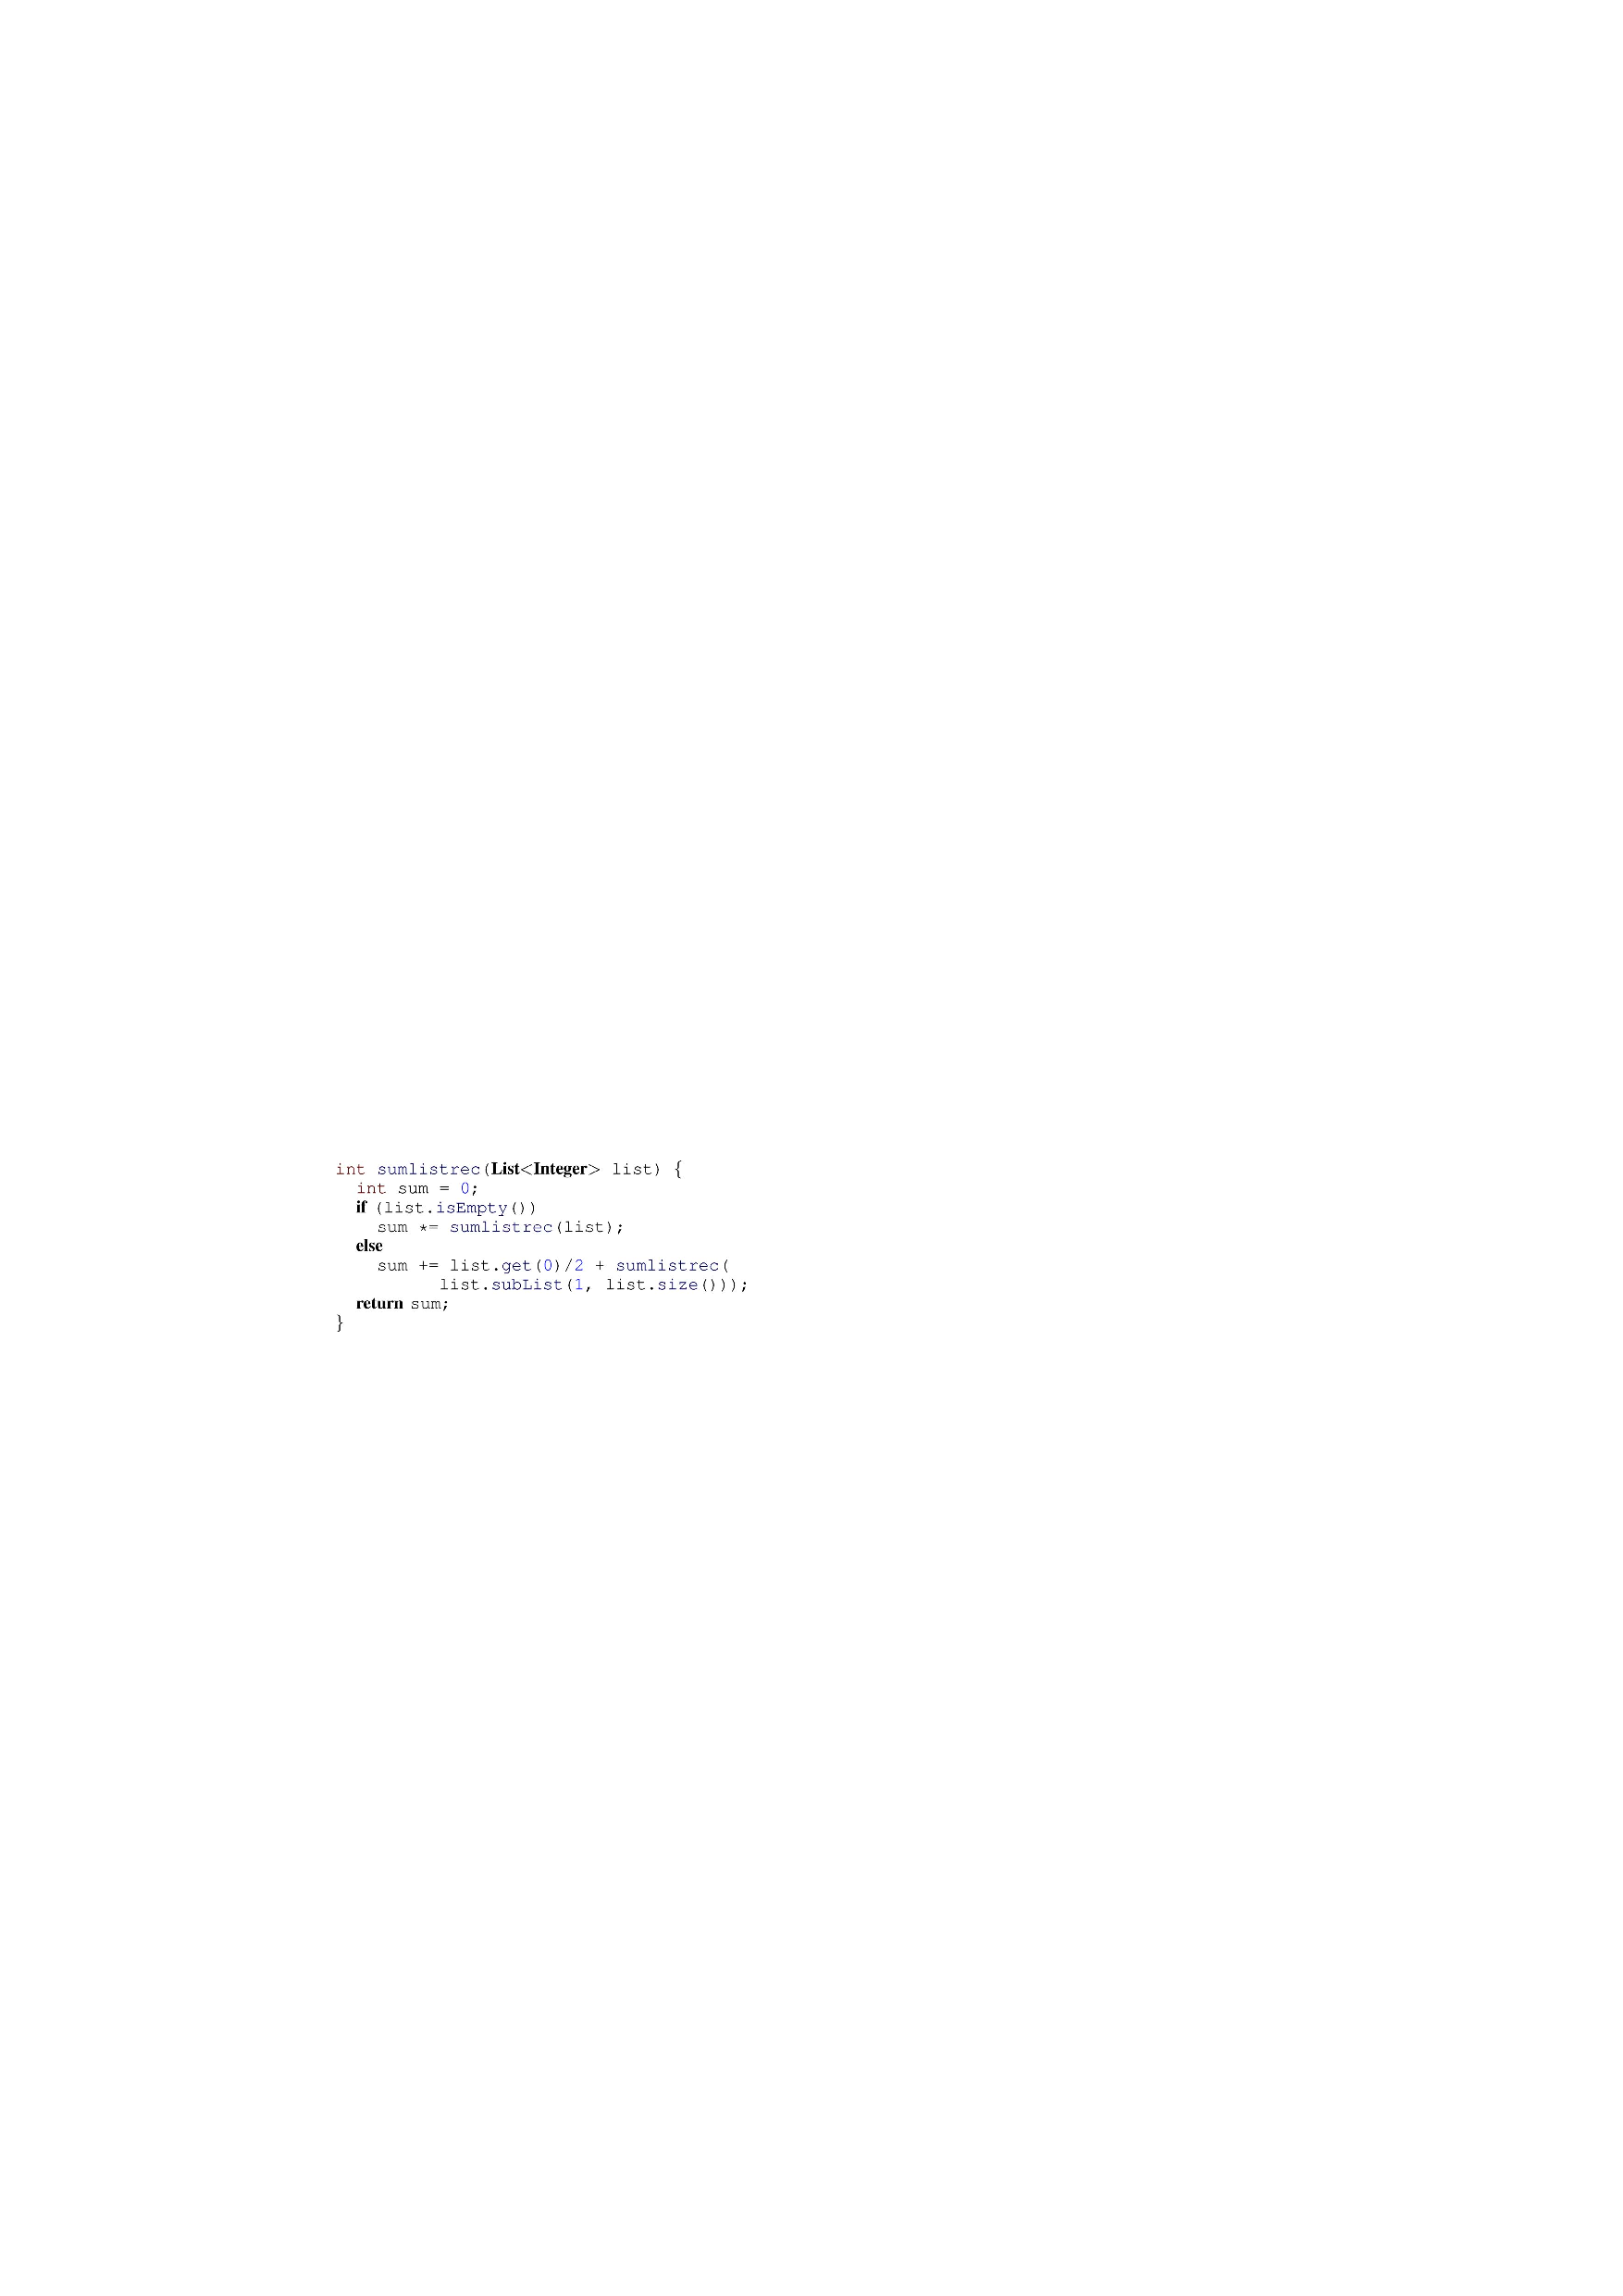
\psfig{file=infrec.pdf}
\caption{Initial population function, for the array sum problem, before being compiled to Java bytecode to be evolved.This function enters into infinite recursion in the if statement. Taken from ~\cite{FINCH:2011}.}
\label{initial rec}
\end{figure}

\begin{figure}
\centering
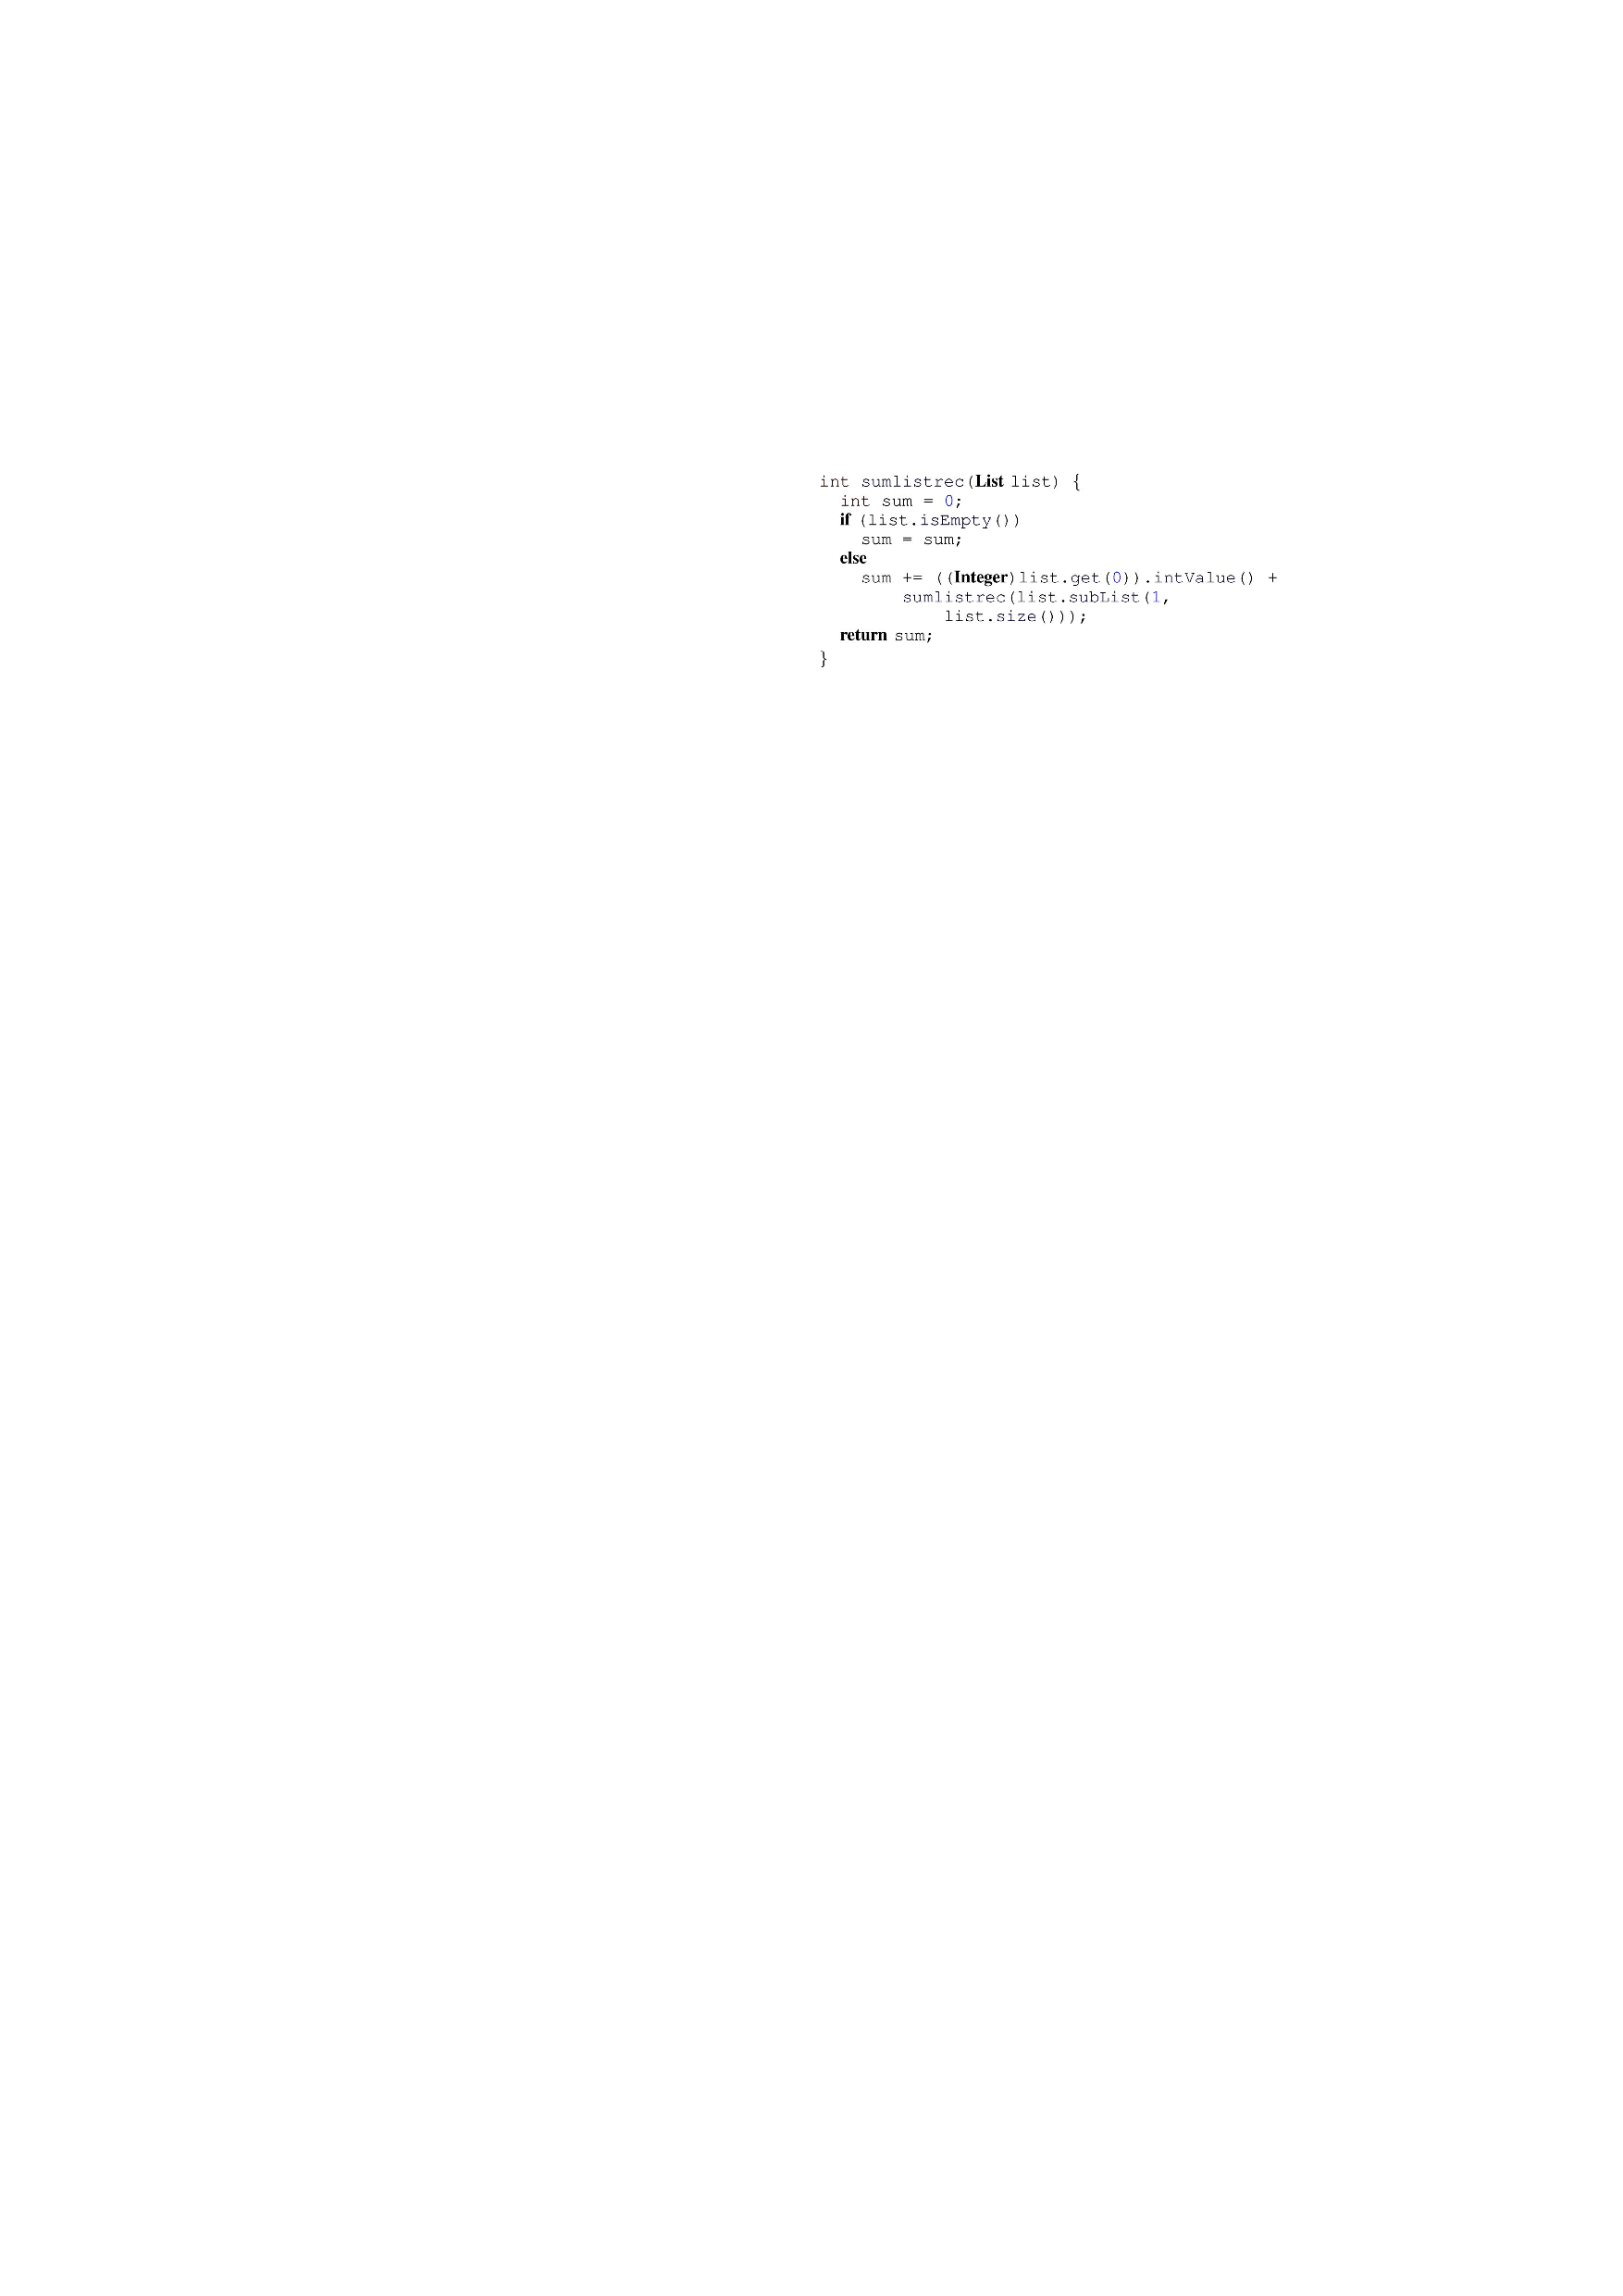
\psfig{file=recsolution.pdf}
\caption{FINCH's decompiled solution to the initial program presented in Figure~\ref{initial rec}. Taken from ~\cite{FINCH:2011}.}
\label{final rec}
\end{figure}

\subsubsection{Array Sum}
The array sum problem consists of adding up all the values in an array. This problem is important because it requires evolving a loop or recursion to find a solution. This would show that FINCH is capable of evolving more complex programs. FINCH was able to produce a solution to this problem using both recursion and loops. It was also shown that FINCH was able to apply evolution to different list abstractions such as List and ArrayList.

When evolving array sum with recursion the initial population consisted of an individual who entered infinite recursion as shown in Figure \ref{initial rec}. Due to the way FINCH deals with non-halting programs, this was not a problem and evolution ensued. The resulting code from evolving Figure \ref{initial rec} is shown in Figure \ref{final rec}.


\subsection{Automated Bug Repair}

Schulte et al.,~\cite{Assembly:2010} were able to show that it is possible to fix human programming errors by evolving instruction-level code. They were able to successfully debug various programs containing bugs such as infinite loops and buffer overflow. The interesting thing about these experiments was that they were performed on programs written by software developers and at times the programs consisted of thousands of lines of code. Some bugs that were fixed through the evolution of instruction-level code were not possible in their previous work~\cite{Forrest:2009} with source code. For example, their EA in their previous work was not capable of fixing incorrect type declarations. This suggests it is easier to repair a wider array of bugs by evolving instruction-level code.

Although a considerable number of offspring with a fitness of zero were produced, this did not seem to damage the result. The average number of fitness evaluations required to produce an offspring that passed all the tests was 74.4 for assembly compared to 63.6 for C from previous work~\cite{Forrest:2009}. This indicates that computational work needed to evolve repairs in assembly is comparable to that of source code. Even programs that contained thousands of lines of code only required a few generations. Thus, using instruction-level evolution to automate bug repair is feasible.
 

\section{Conclusions and Future Work}

\subsection{Future Work}


Future work may include evolving programs whose solutions are much longer and more complicated. Orlov and Sipper~\cite{FINCH:2011} proved that by applying GP to bytecode it is possible to solve many simple problems. However, most of the solutions only consisted of a small number of lines of code. It would be exciting to see something more complex be evolved. Also, as shown in Figure~\ref{final rec} a solution given by FINCH might not be clearly legible once decompiled back to source code. Refactoring would have to be done to make the code more readable and maintainable.

An extension of future work, using the research in \cite{Assembly:2010}, could include debugging on less focused areas, such as attempting to fix bugs that require multiple fixes throughout the code rather than simply altering one line. Also, there is the question of how applicable automated bug repair is in a real world situation. In most real world scenarios test coverage is very minimal and would rarely cover the entire code base. Some changes to a program could cause it to break. If test cases do not cover that case then a fix to the original bug could contain a different bug. 


\subsection{Conclusion}
Evolving entire programs at the instruction-level is possible at the source code level. No assumptions about the program being evolved is needed, and it is easier to deal with the semantic constraints. Schulte et al., and ~\cite{Assembly:2010, FINCH:2011} showed that evolving instruction-level code is just as feasible as source code and at times better, such as for debugging incorrect type declarations. In conclusion, evolving instruction-level code is feasible and exciting for the field of EC. It opens up many possibilities that were once unavailable.
%\end{document}  % This is where a 'short' article might terminate

%ACKNOWLEDGMENTS are optional
\section*{Acknowledgments}
A special acknowledgment to Nic McPhee and Elena Machkasova for their time and knowledge. Also, thanks to Debra Dogotch, Chris Thomas, Peter Dolan, and Tim Snyder.

%
% The following two commands are all you need in the
% initial runs of your .tex file to
% produce the bibliography for the citations in your paper.
\bibliographystyle{abbrv}
\bibliography{EricBibliography}  % ElenaSample.bib is the name of the Bibliography in this case
% You must have a proper ".bib" file
%  and remember to run:
% latex bibtex latex latex
% to resolve all references
%
% ACM needs 'a single self-contained file'!
%
%APPENDICES are optional
%\balancecolumns

\end{document}

\appendix
%Appendix A
\section{Headings in Appendices}
The rules about hierarchical headings discussed above for
the body of the article are different in the appendices.
In the \textbf{appendix} environment, the command
\textbf{section} is used to
indicate the start of each Appendix, with alphabetic order
designation (i.e. the first is A, the second B, etc.) and
a title (if you include one).  So, if you need
hierarchical structure
\textit{within} an Appendix, start with \textbf{subsection} as the
highest level. Here is an outline of the body of this
document in Appendix-appropriate form:
\subsection{Introduction}
\subsection{The Body of the Paper}
\subsubsection{Type Changes and  Special Characters}
\subsubsection{Math Equations}
\paragraph{Inline (In-text) Equations}
\paragraph{Display Equations}
\subsubsection{Citations}
\subsubsection{Tables}
\subsubsection{Figures}
\subsubsection{Theorem-like Constructs}
\subsubsection*{A Caveat for the \TeX\ Expert}
\subsection{Conclusions}
\subsection{Acknowledgments}
\subsection{Additional Authors}
This section is inserted by \LaTeX; you do not insert it.
You just add the names and information in the
\texttt{{\char'134}additionalauthors} command at the start
of the document.
\subsection{References}
Generated by bibtex from your ~.bib file.  Run latex,
then bibtex, then latex twice (to resolve references)
to create the ~.bbl file.  Insert that ~.bbl file into
the .tex source file and comment out
the command \texttt{{\char'134}thebibliography}.
% This next section command marks the start of
% Appendix B, and does not continue the present hierarchy
\section{More Help for the Hardy}
The sig-alternate.cls file itself is chock-full of succinct
and helpful comments.  If you consider yourself a moderately
experienced to expert user of \LaTeX, you may find reading
it useful but please remember not to change it.
%\balancecolumns % GM June 2007
% That's all folks!
\end{document}
